\section{Joanna Gorczyca}

Look at this axolotl (see Figure~\ref{fig:axolotl_pink}).

\begin{figure}[htbp]
    \centering
    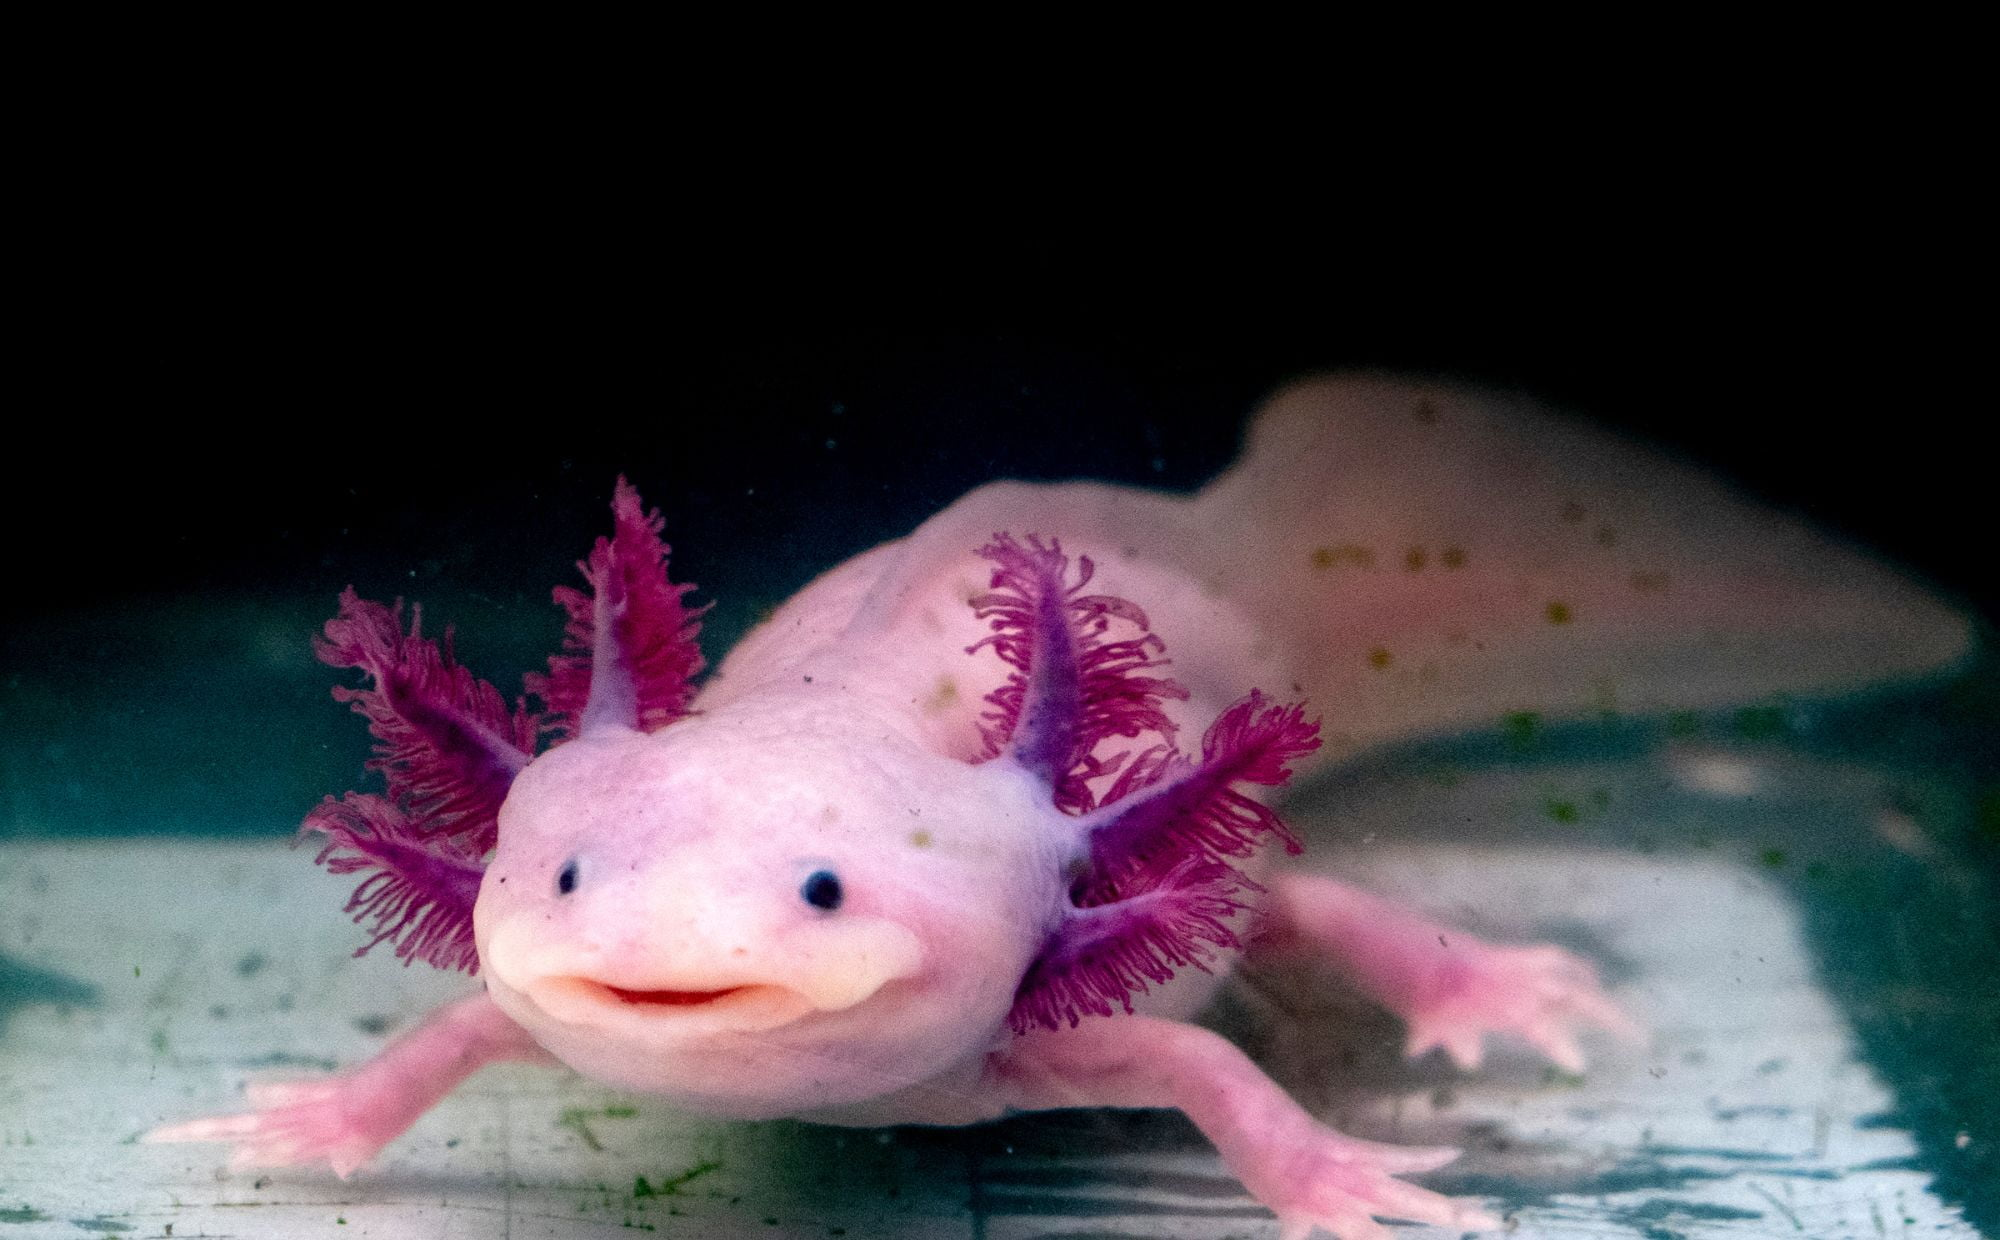
\includegraphics[width=1\textwidth]{pictures/axolotl_pink.jpg}
    \caption{It is very cute.}
    \label{fig:axolotl_pink}
\end{figure}

Some people call this equation the most remarkable formula in mathematics: \[e^{i \pi} + 1 = 0\]

A formula that can be used to draw a heart:
$ (x^{2}+y^{2}+-1)^{3}-x^{2}y^{3}=0 $

\newpage

Axolotl diets \textbf{can be successfully varied}, so long as nutritional benefits and potential detriments are considered. \underline{Below} is a list of potential foods that may be occasionally supplemented, including foods for hatchlings and under-researched crustaceans that may be fed.

Blackworms and tubifex worms are the primary high-protein diet preferred for hatchling axolotls, however, using earthworms and brine shrimp in excess tends to result in healthier axolotls. The reason for this is currently unknown, however, it may be tied to the calcium to phosphorus ratio required by axolotls, which is 2:1. \textbf{Crustaceans are a popular choice for introducing high levels of calcium into the diet}, however, care must be taken to prevent internal impaction caused by high fiber and chitin diets.

% Please add the following required packages to your document preamble:
% \usepackage[table,xcdraw]{xcolor}
% Beamer presentation requires \usepackage{colortbl} instead of \usepackage[table,xcdraw]{xcolor}
\begin{table}[htbp]
\caption{\textbf{Data on the nutritional content of additional food options.}} 


\begin{tabular}{
>{\columncolor[HTML]{FFFFFF}}l 
>{\columncolor[HTML]{FFFFFF}}l 
>{\columncolor[HTML]{FFFFFF}}l 
>{\columncolor[HTML]{FFFFFF}}l 
>{\columncolor[HTML]{FFFFFF}}l }
             & Protein \% & Fat \% & Calcium \% & Ca:P \\
Tubifex      & 46.1       & 15.1   & 0.19       & 0:26 \\
Blackworm    & 47.8       & 20.1   & 0.11       & 0:12 \\
White Worm   & 70         & 14.5   & N/A        & N/A  \\
Grindal Worm & 70         & 14.5   & N/A        & N/A  \\
Daphnia      & 55.2       & 6.6    & 0.1        & 0.08 \\
Brine Shrimp & 55         & 14     & 5          & N/A  \\
Springtails  & 55.4       & 28     & 26.9       & N/A  \\
Scuds        & 40         & 5.5    & 4.1        & N/A  \\
Bloodworms   & 52.8       & 9.7    & 0.38       & 0:42 \\
Isopods      & 41.2       & 11.5   & 14.38      & 12:1
\end{tabular}
\end{table}
\href{https://www.axolotlcentral.com/post/axolotl-nutrition}{Source: www.axolotlcentral.com/post/axolotl-nutrition} \\

\textbf{Where do axolotl live?} \\
Axolotls are exclusively found in two freshwater lakes in Mexico 
\begin{enumerate}
    \item One Lake Xochimilco 
    \item Two Lake Chalco
\end{enumerate} 
\textbf{Why are axolotls endangered?}
\begin{itemize}
  \item Water pollution
  \item Overfishing
  \item Habitat loss
  \item Invasive species
\end{itemize}